\documentclass
[10pt, xcolor=dvipsnames]
%[11pt,compress ,xcolor=dvipsnames]
{beamer}

\usepackage{graphicx}
\graphicspath{ {../figures} }

\usepackage{caption}
\captionsetup[figure]{font=scriptsize,labelfont=scriptsize}
\captionsetup[table]{font=scriptsize,labelfont=scriptsize}

% justified text
\renewcommand{\raggedright}{\leftskip=0pt \rightskip=0pt plus 0cm}

% overlays
%\setbeamercovered{transparent}

% bibliography 

\usepackage[utf8]{inputenc}
\usepackage[english]{babel}
%\usepackage[
%    style=alphabetic, 
%    backend=bibtex,
%    sorting=none
%    ]{biblatex}
%\bibliography{ref}{}
%\renewcommand*{\bibfont}{\scriptsize}

% Removes icon in bibliography
%\setbeamertemplate{bibliography item}{\hspace{-4em}}

\usepackage{amsmath}
\usepackage{braket}
\usepackage{booktabs}
\usepackage{tikz}
\usepackage{adjustbox}
\usepackage{verbatim}
\usepackage{setspace}
\usepackage{subcaption}

\usepackage[] %qm
{qcircuit}
% theme


\useoutertheme[]{infolines} % Alternatively: miniframes, infolines, split
%\usecolortheme{whale}
%\usetheme{CambridgeUS}
\useinnertheme{circles}
%
\definecolor{UBCblue}{rgb}{0.04706, 0.13725, 0.26667} % UBC Blue (primary)
\definecolor{UBCgrey}{rgb}{0.3686, 0.5255, 0.6235} % UBC Grey (secondary)
\definecolor{light-grey}{RGB}{240,240,240}

\setbeamercolor{palette primary}{bg=UBCblue,fg=white}
\setbeamercolor{palette secondary}{bg=UBCblue,fg=white}
\setbeamercolor{palette tertiary}{bg=UBCblue,fg=white}
\setbeamercolor{palette quaternary}{bg=UBCblue,fg=white}
\setbeamercolor{structure}{fg=UBCblue} % itemize, enumerate, etc
\setbeamercolor{section in toc}{fg=UBCblue} % TOC sections
\setbeamercolor{subsection in head/foot}{bg=UBCgrey,fg=white}
\setbeamercolor{title}{bg=UBCblue,fg=white}
\setbeamercolor{block title}{bg=UBCgrey,fg=white}
\setbeamercolor{block body}{bg=light-grey, fg=black}
\setbeamercolor{frametitle}{bg=light-grey,fg=black}


% ------- DOCUMENT --------

\title[The pizza guy]{The pizza guy problem using Minizinc}
\author[Boldini, Diana, Zaglio]{G. Boldini, A. Diana, F. Zaglio}
\institute[UNIPR]{University of Parma\newline
    Master's Degree in Computer Science\newline
    Constraint Programming}
\date{AA 2021/22}


\newcommand\blfootnote[1]{%
  \begingroup
  \renewcommand\thefootnote{}\footnote{#1}%
  \addtocounter{footnote}{-1}%
  \endgroup
}


\AtBeginSection[]{
	\begin{frame}{Outline}
		\tableofcontents[sectionstyle=show/shaded,subsectionstyle=show/shaded/hide,subsubsectionstyle=show/shaded/hide]
	\end{frame}
}



\begin{document}

% interlinea
%\linespread{1.5}
%\doublespacing


\setbeamertemplate{navigation symbols}{}


% title 
\begin{frame}[plain]
    \titlepage
\end{frame}
\addtocounter{framenumber}{-1}


% outline
\begin{frame}{Outline}
    \tableofcontents[sectionstyle=show,subsectionstyle=show/shaded/hide,subsubsectionstyle=show/shaded/hide]
%    \tableofcontents
\end{frame}


\section{Introduction}

\begin{frame}[allowframebreaks]
    {The pizza guy problem}
    The best pizzeria in the town delivers pizzas at home and we want to find:
    \begin{itemize} 
        \item the best schedule of the set of orders,
        \item minimize the total traveled distance by all the deliverers, 
        \item respect the delivery times requested by the customers.
    \end{itemize}
    \vspace{0.3cm}
    Solving the problem means:
    \begin{itemize}
        \item assign a set of sorted lists of orders to every deliverer,
        \item where each list represents an "ordered" travel.
    \end{itemize}
    \pagebreak
    \begin{enumerate}
		\item An \textit{order} consists in:
		\begin{enumerate}
			\item a delivery address,
			\item a desired delivery time (granularity of 15 minutes) from 19.00 to 22.00,
			\item a number of pizzas.\\~\
		\end{enumerate}
        \item Delivery window:
        \begin{enumerate}
			\item is up to 30 minutes later than desired delivery time;
			\item during this time, multiple travels from and to the pizzeria are allowed.\\~\
		\end{enumerate}

		\item The street topology of the city can be seen as a graph (the edges rappresent the travel time).\\~\
		\item Max pizza carried by a deliverer: 16.
		
	\end{enumerate}
\end{frame}

\section{Model}
\begin{frame}{Input Data}
    The input consists in having:
	\begin{enumerate}
		\item $d$: number of deliverers,
		\item $mdist$: 2-d matrix representing the travel distance between
			every pair of nodes (with Dijkstra),
		\item $k$: side dimension of $mdist$,
		\item a set of $N$ orders, each of them made by a destination $dest$, a delivery 
			time $orario$ and a number of pizzas $num\_pizzas$:
            
			\begin{equation*}
				\begin{split}
					\text{orario} &= [o_1, o_2, \dots, o_N];\\
					\text{num\_pizzas} &= [np_1, np_2, \dots, np_N];\\
					\text{dest} &= [d_1, d_2, \dots, d_N];
				\end{split}	
			\end{equation*}
	\end{enumerate}
\end{frame}
\begin{frame}{Assumptions}
	\begin{enumerate}
		\item the graph could be undirected;\\~\
		\item a deliverer can do only a single travel 
        (from pizzeria, to all destination nodes and back to pizzeria) in one half-an-hour ($h$);
        \begin{itemize}
            \item the total number of $h$ is 6 (\# slots in 19.00 - 22.00)\\~\
        \end{itemize}
            
		\item distances and travels time are considered the same thing;\\~\
		\item the set of orders is known before the start of the evening;\\~\
		\item all the time needed by the deliverer to interacts with customers
                 is supposed to be zero. 
	\end{enumerate}
\end{frame}

\begin{frame}[allowframebreaks]{Implementation}
    $d$ : \# deliverers, $N$: \# deliveries and $h$: \# time slots.\\~\

    As decisional variables, we used these following data structures:
    \begin{itemize}
		\item {scheduling:\\
            \begin{center}
                \texttt{array[1..d, 1..N, 1..h] of var bool: scheduling;}
            \end{center}    
        }
        \item {P: destinations to reach\\
            \begin{center}
                \texttt{array[1..d, 1..N, 1..h] of var array2set(dest) union {0}: P;}
            \end{center}
        }
		\item {X: position of destinations to reach\\
            \begin{center}
                \texttt{array[1..d, 1..N, 1..h] of var 0..N: X;}
            \end{center}
        }
        \item {distances\\
            \begin{center}
                \texttt{array[1..d, 1..N, 1..h] of var 0..29: distances;}
            \end{center}
        }
        \pagebreak
		\item {pizza\_carried\\
            \begin{center}
                \texttt{array[1..d, 1..h] of var 0..16: pizzas\_carried;}
            \end{center}
        }
		\item {estimated arrival (ea)\\
            \begin{center}
                \texttt{array[1..N] of var 0..h*30: ea;}
            \end{center}
        }
		
		\item {total\_travel\\
            \begin{center}
                \texttt{array[1..d, 1..h] of var 0..29: total\_travel;}
            \end{center}
        } 
	\end{itemize}
\end{frame}

\begin{frame}[fragile]{Constraints: scheduling and P consistency}
    Scheduling consistency:
    \begin{itemize}
		\item ensures that all the orders are fulfilled: \\
            \begin{center}
                \texttt{sum(scheduling) = N;}
            \end{center}
            
		\item ensures that only one delivever takes care of one order:
          \begin{center}
            \texttt{forall(j in 1..N)(\\
			    sum([scheduling[id,j,ih]| id in 1..d, ih in 1..h]) = 1\\
		  );}
        \end{center}
        \end{itemize}
    \vspace{0.5cm}
    P construction: 
    \begin{verbatim}
    forall(id in 1..d, iN in 1..N, ih in hra[iN])(
        P[id, iN, ih] = scheduling[id, iN, ih] * dest[iN]
    );
    \end{verbatim}
\end{frame}

\begin{frame}[fragile]{Constraints: X consistency}
    X has to contain all the meaningful positions in P:
    \begin{verbatim}
    forall(id in 1..d, iN in 1..N, ih in 1..h)(
        if P[id, iN, ih] > 0 then 
            count([ X[id, iNN, ih] | iNN in 1..N], iN, 1)
        else
        (
            count([ X[id, iNN, ih] | iNN in 1..N], iN, 0) 
            /\
            distances[id,iN,ih] = 0
        )
        endif
    );
    \end{verbatim}
    Also, for each row of X, we want to push all the meaningless values (zeros) to the end
    (done in another constraint).
\end{frame}

\begin{frame}[fragile]{Constraints: distances calculation}
    Considering a single row of \texttt{X}, two different cases:
    \begin{itemize}
        \item the first (meaningful) cell;
        \item all the others (meaningful) cells.
    \end{itemize}
\begin{verbatim}
    forall(id in 1..d, iN in 1..N, ih in 1..h)(
        if X[id,iN,ih] !=0 then
           if iN == 1 then
              distances[id, X[id,iN,ih], ih] = 
                 mdist[1, P[id, X[id,iN,ih], ih]] 
            else
               distances[id, X[id,iN,ih], ih] = 
                 mdist[P[id, X[id,iN-1,ih], ih], P[id, X[id,iN,ih], ih]] 
                  + distances[id,X[id,iN-1,ih], ih]
                       | iNN in 1..iN-1])
            endif
        endif
     );
\end{verbatim}

\end{frame}

\begin{frame}[fragile]{Constraints: total travel}
    
    Total travel consistency ensured by \texttt{total\_travel} domain of \texttt{[0..29]}:
    
    \begin{verbatim}
    constraint forall(id in 1..d, iN in 1..N, ih in 1..h)(
        ( X[id,iN,ih] !=0
            /\ ( iN+1 == N+1 \/ X[id,iN+1,ih] == 0)
            /\ P[id,X[id,iN,ih],ih] != 0)

            -> (total_travel[id,ih] = 
                distances[id, X[id,iN,ih], ih] 
                + mdist[P[id, X[id,iN,ih], ih],1])   
    );
    \end{verbatim}

    
\end{frame}

\begin{frame}[fragile]{Constraints: ea \& pizza\_carried}

Expected arrival: all the orders must arrive in the delivery window.
    \begin{verbatim}
forall(iN in 1..N)(
   ea[iN] = sum([scheduling[id,iN,ih]
            * (distances[id,iN,ih]+((ih-1)*30)) 
               | id in 1..d, ih in 1..h])
   /\ ea[iN] >= ra[iN] 
   /\ ea[iN] < ra[iN]+30 
);
    \end{verbatim}

Number of pizzas carried for each travel:
    \begin{verbatim}
forall(id in 1..d, ih in 1..h)(
   pizzas_carried[id, ih] = sum([ num_pizze[j]
                                | j in 1..N 
                                where scheduling[id, j, ih] = 1])
);
    \end{verbatim}
\end{frame}


\begin{frame}{Graphical representation}

    \begin{center}
        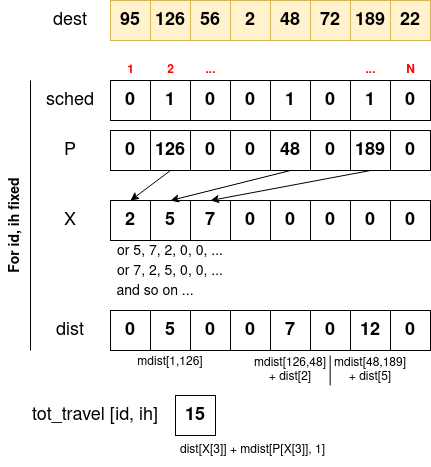
\includegraphics[scale=.45]{drawio.png}
    \end{center}

\end{frame}

\begin{frame}[fragile]{Restrict the search space}

    \begin{enumerate}
        \item domain restrictions;
        \item for each order, exclude all the non-possible half-an-hour;
        \begin{verbatim}
    forall(id in 1..d, iN in 1..N, ih in (1..h diff hra[iN]))(
        scheduling[id,iN,ih] = 0
        /\ P[id,iN,ih] = 0
        /\ distances[id,iN,ih] = 0
        /\ count( [X[id,iNN,ih] | iNN in 1..N], iN, 0)
    );
        \end{verbatim}
        \item enforce useless cells of \texttt{X} to be zero (and push them to the bottom).
  \begin{verbatim}
    forall(id in 1..d, ih in 1..h)(
        let {
            var int: c = count([P[id,iNN,ih] | iNN in 1..N],0)
        } in forall(iN in N-c+1..N)(
            X[id,iN,ih] = 0
            )
    );
  \end{verbatim}
\end{enumerate}

\end{frame}

\begin{frame}[fragile]{Symmetry breaking}

    Simmetry $\rightarrow$ having multiple deliveriers.\\~\

    \textit{e.g.} 3 orders, 2 deliverer (\texttt{d1} and \texttt{d2}).\\
    \hspace{1em}best strategy: first two togheter, third alone.\\

    \hspace{1em}$\rightarrow$ first two can be assigned to \texttt{d1} and the third to \texttt{d2}\\
    \hspace{2em} and \textbf{viceversa}. \\~\

Impose an order on the deliverers:

\begin{verbatim}
forall(ih in 1..h, id in 1..d-1)(
    pizzas_carried[id,ih] >= pizzas_carried[id+1,ih]
);
\end{verbatim}

\end{frame}

\section{Results}


\begin{frame}{Tests and results}
    

    Different analyzes:
    \begin{itemize}
        \item search strategies comparison;
        \item same problem with different cities (of increasing size);
        \item same city, increasing complexity of the problem;
        \item real-world application.\\~\
    \end{itemize}

    5 real-world italian cities considered:
    \begin{table}[h]
		\centering
		\begin{tabular}{l|ll}
			City & nodes & edges \\
			\hline
			Visano & 297 & 378 \\
			Asola & 480 & 664 \\
			Montichiari & 1130 & 1509 \\
			Brescia & 3925 & 5464 \\
			Roma & 4729 & 7277 \\
		\end{tabular}		
	\end{table}
	
    \texttt{mdist} computed using Dijkstra as pre-preprocessing step.


\end{frame}




\begin{frame}{Search strategies comparison}

    \begin{center}
		$N = 12$ (orders), $d = 2$ (deliverers), city = Visano.	\\~\	
	\end{center}

    Changing the search annotations:
    \begin{itemize}
        \item the search variable;
        \item how the variable is choosen (VCA);
        \item how to constraint the variable (VSA).\\~\
    \end{itemize}

    Result:
    \begin{itemize}
        \item searching of variable \texttt{scheduling} is usually faster;
        \item some VCA (Variable Choice Annotation) and
        VSA (Variable Search Annotation) appear to be more promising 
        than others.
    \end{itemize}
\end{frame}

\begin{frame}{Search strategies comparison: preliminary analysis}
    \begin{figure}
		\centering

		\begin{subfigure}[b]{.3\textwidth}
			\centering
			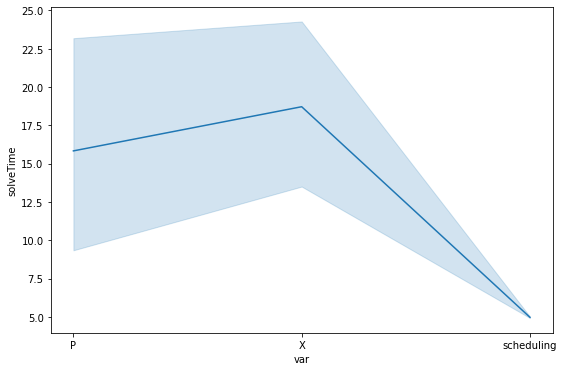
\includegraphics[width=\textwidth]{var.png}
			\caption{changing search variable.}
		\end{subfigure}
		\begin{subfigure}[b]{.69\textwidth}
			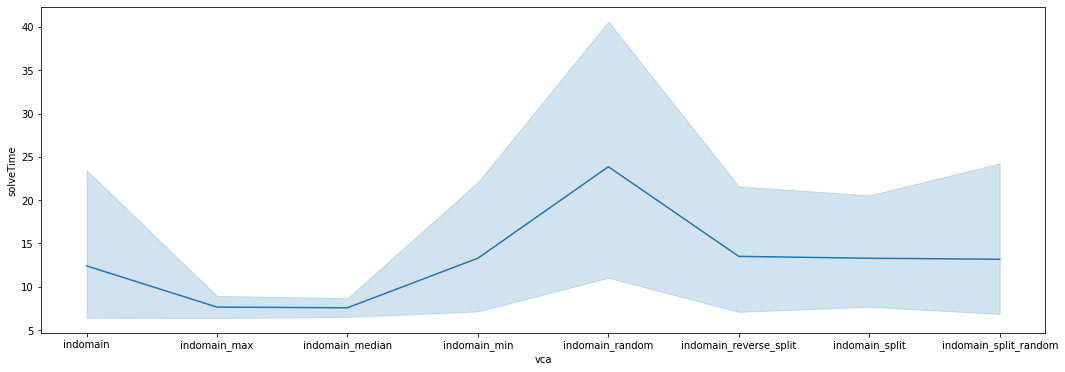
\includegraphics[width=.9\textwidth]{vca.png}
			\caption{changing Variable Choice Annotation (VCA)}
		\end{subfigure}
		\begin{subfigure}[b]{\textwidth}

            \centering
            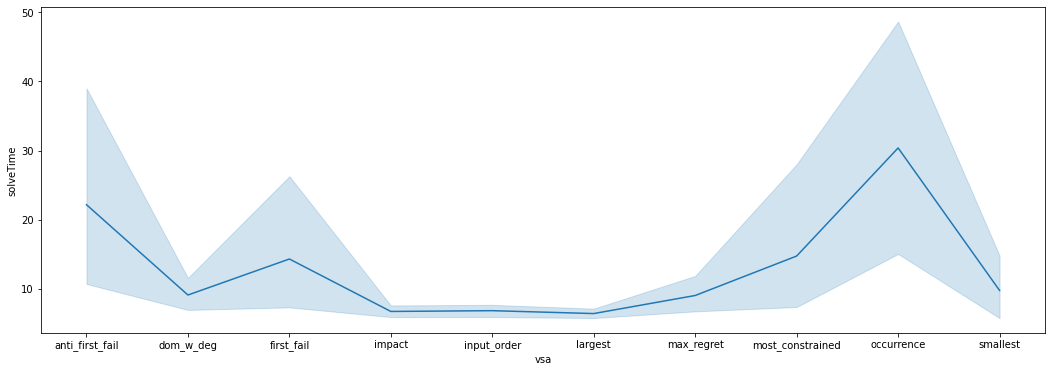
\includegraphics[width=.8\textwidth]{vsa.png}
			\caption{changing Variable Search Annotations (VSA)}
		\end{subfigure}
		
	\end{figure}
 
\end{frame}

   
    %\includegraphics{}{var.png}



\begin{frame}[allowframebreaks]{Search strategies comparison: more specific analysis}

    Subset of search strategies (the most promising) considered.\\
    Timeout of 20 seconds.\\~\

    Correlation matrix:
    \begin{itemize}
        \item number of failures and number of nodes (1)
        \item number of propagations and solve time (0.79) and 
        non-correlation between maximum depth and solve time (-0.05)
    \end{itemize}

    \begin{figure}
        \centering
        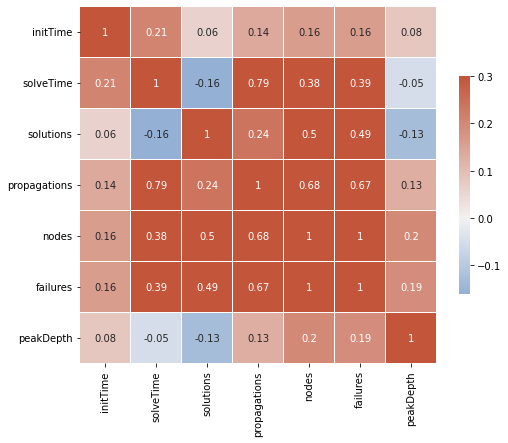
\includegraphics[width=.3\textwidth]{corr.png}
    \end{figure}

    \framebreak

    \begin{figure}
		\centering
		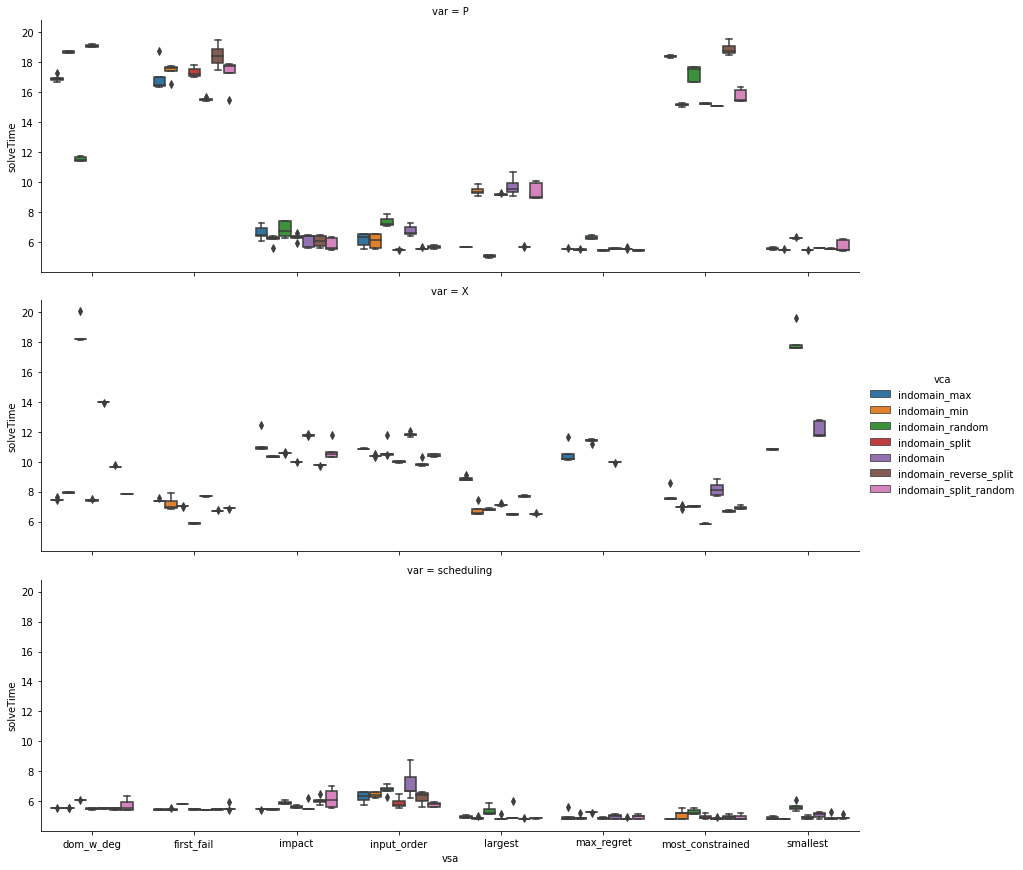
\includegraphics[width=.72\textwidth]{solve-time-specific.png}
	\end{figure}

\end{frame}

\begin{frame}{5 city of increasing size}

    \begin{center}
		$N = 12$ (orders), $d = 2$ (deliverers), changing the city
	\end{center}


    \begin{figure}
		\centering
		\begin{subfigure}[c]{.49\textwidth}
			\centering
			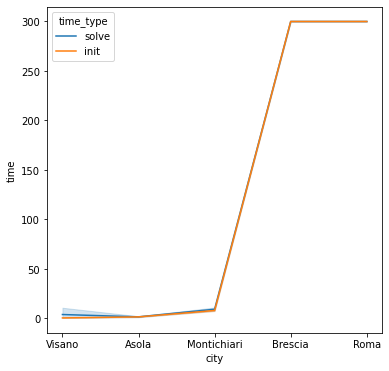
\includegraphics[width=.7\textwidth]{city-increasing-size.png}
		\end{subfigure}
		\begin{subfigure}[c]{.49\textwidth}
			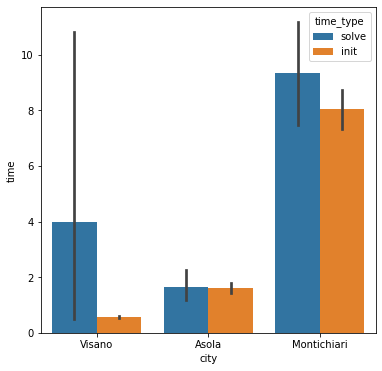
\includegraphics[width=.7\textwidth]{city-increasing-size-2.png}

		\end{subfigure}
	\end{figure}

    Roma and Brescia always reach timeout.

\end{frame}

\begin{frame}[allowframebreaks]{Changing the complexity of the problem}

    $N = 2\dots15,\hspace{.5em} d=1\dots4$, city = Visano, 2 minutes timeout.\\~\

    \begin{figure}
        \centering
		\begin{subfigure}[c]{\textwidth}
            \centering
			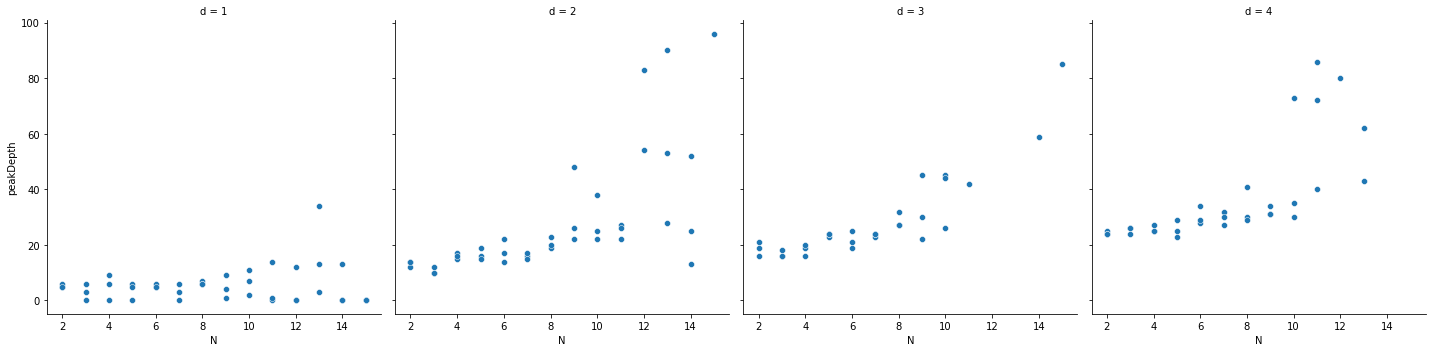
\includegraphics[width=.8\textwidth]{incr-problem-depth.png}
			\caption{peakDepth}
		\end{subfigure}
		\begin{subfigure}[b]{\textwidth}
            \centering
			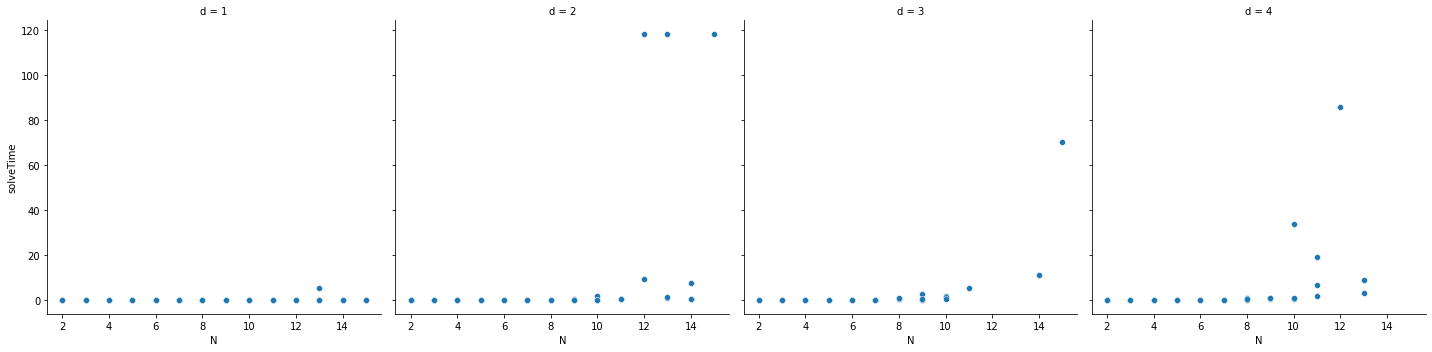
\includegraphics[width=.8\textwidth]{incr-problem-time.png}
			\caption{Solve time}
		\end{subfigure}
		\begin{subfigure}[b]{\textwidth}
            \centering
			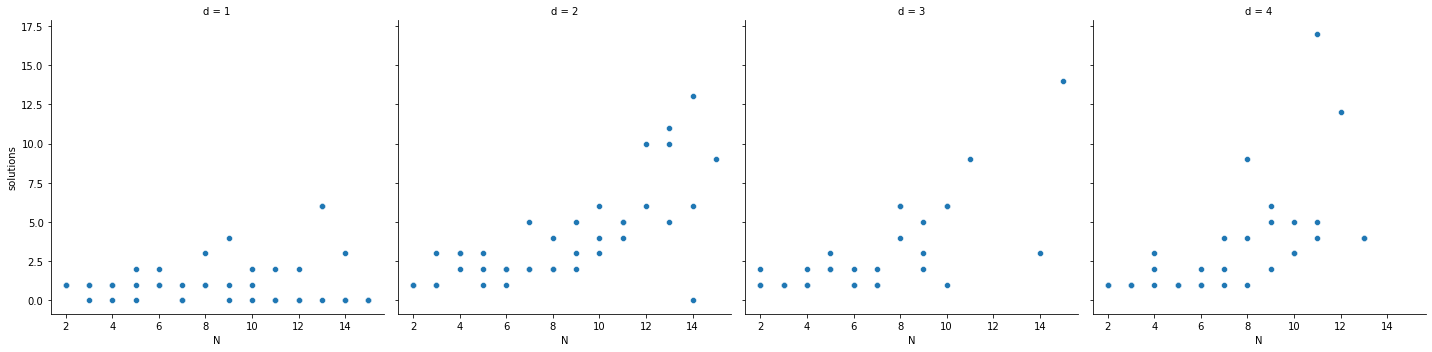
\includegraphics[width=.8\textwidth]{incr-problem-solutions.png}
			\caption{Solutions}
		\end{subfigure}
		\begin{subfigure}[b]{\textwidth}
            \centering
			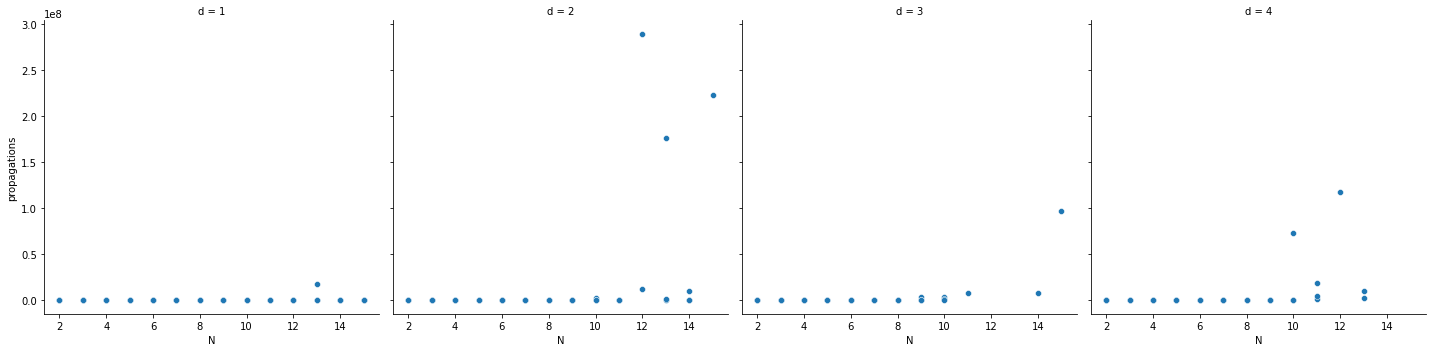
\includegraphics[width=.8\textwidth]{incr-problem-propagations.png}
			\caption{Propagations}
		\end{subfigure}

	\end{figure}
\end{frame}

\begin{frame}{Real world application}

    City graph from \texttt{OpenStreetMap (Python)}.\\
    \texttt{mdist} filled with Dijkstra.\\~\

    \begin{figure}
		\begin{subfigure}[t]{.5\textwidth}
			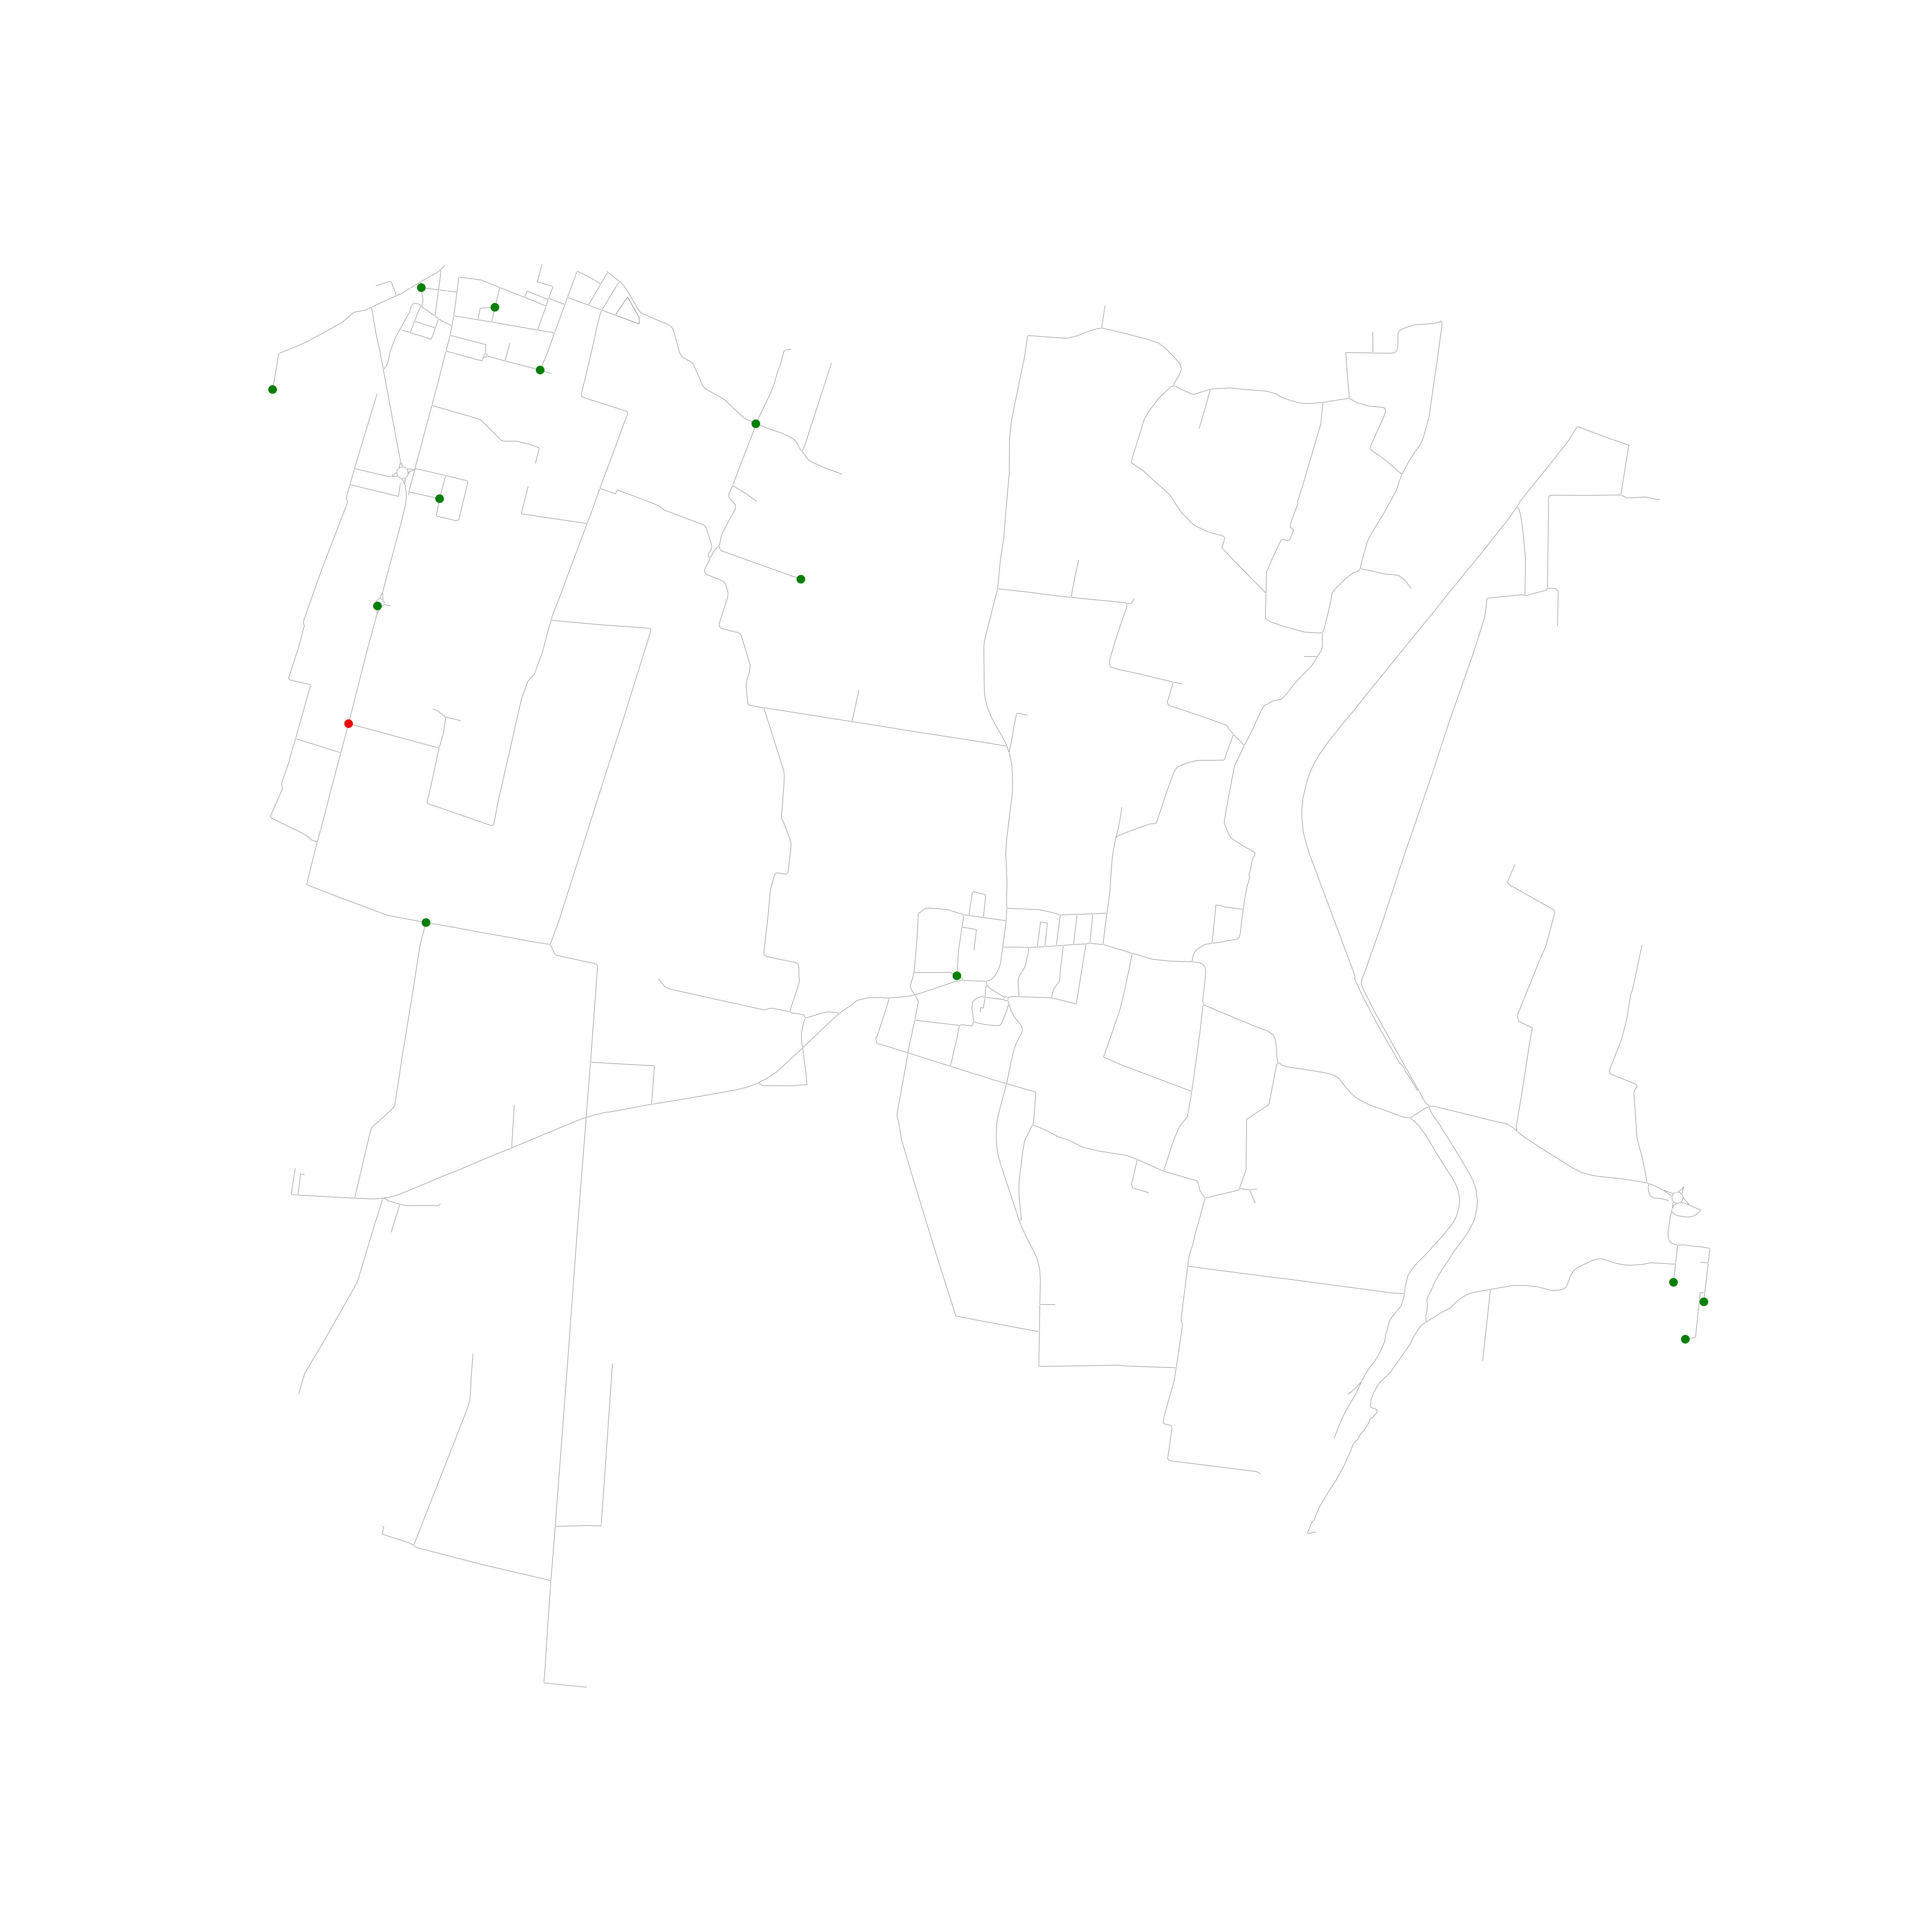
\includegraphics[width=.7\textwidth]{graph.png}
			\caption{Pizzeria (red) and destinations to reach (green)}

		\end{subfigure}
		\begin{subfigure}[t]{.49\textwidth}
			\includegraphics[width=.7\textwidth]{graph_paths-min.png}
			\caption{Path for each deliverer}
		\end{subfigure}
	\end{figure}



    \textit{Visano}, $N = 13$, $d = 2$, solve time: 48.8 seconds.

\end{frame}

\section{Conclusions}

\begin{frame}{Conclusions}
    \begin{enumerate}
        \item Our proposed model seems to work.\\~\
        \item \textit{But} the time increases quickly with the size of the problem:
        \begin{itemize}
            \item timeout of 5 minutes for $N \ge 15$ and $d \ge 3$ 
            \item real-world scenario: $N \ge 60, d \ge 3$\\~\
        \end{itemize}
        \item Worst results with the other solvers besides Gecode. \\~\
    \end{enumerate}

    Possible improvements:
    \begin{itemize}
        \item reduce \texttt{mdist} size (already done but not reported);
        \item balancing function between deliverers could be useful;
        \item find a way to exclude two destinations that are too far away from the same travel;
        \item maybe rethink about the model.
    \end{itemize}

\end{frame}

\begin{frame}
    \huge Thank you.
    \begin{figure}
        \hfill
        
\includegraphics[width=.5\textwidth]{diana-pizza-guy.png}
        
    \end{figure}
\end{frame}

%\appendix
%
%% References
%%\nocite{*}
%
%\begin{frame}{Riferimenti}
%    %\fontsize{3}{6}\selectfont
%    \printbibliography[heading=none]
%\end{frame}


\end{document}



%
%\begin{frame}[allowframebreaks]{Algoritmo di Grover \cite{grover1996}}
%
%    Algoritmo di ricerca non strutturato. 
%
%    \begin{figure}
%        \centering
%        \includegraphics[width=.6\textwidth]{grover_list.png}
%    \end{figure}
%    
%    $n$: bit/qubit, $N = 2^n$: spazio di ricerca.\\~\ 
%
%    Per trovare l'elemento \textit{marcato}:
%    \begin{itemize}
%        \item (classico) $N/2$ passi (in media), $N$ (caso pessimo).
%        \item (quantistico - Grover) $\sqrt{N}$ passi $\rightarrow$ speedup quadratico.\\~\
%        
%        %Additionally, the algorithm does not use the list's internal structure, which makes it generic; this is why it immediately provides a quadratic quantum speed-up for many classical problems.
%    \end{itemize}
%
%    Trucco di base: amplificazione dell'ampiezza (usato da diversi algoritmi).
%
%    \framebreak
%
%    Tre fasi:
%    \begin{enumerate}
%        \item Inizializzazione: crea uno stato di sovrapposizione di ogni possibile elemento $\ket{\Psi}$.
%            $$\ket{\Psi} = H^{\otimes n} \ket{0}$$
%        
%        \item \textit{Iterazione di Grover} ripetuta $R = \mathcal{O}(\sqrt{N})$ volte:
%        \begin{itemize}
%            \item Oracolo: applica l'operatore $U_f$ che inverte la fase dello/gli stato/i soluzione/i
%            $$
%            U_f\ket{\Psi} = (-1)^{f(x)} \ket{\Psi}, \text{\hspace*{1em}}
%            f(x) =
%            \begin{cases}
%                0 & x \neq a,\\
%                1 & x = a.
%            \end{cases}
%            $$
%            \item Diffusore: riflette intorno allo stato $\ket{\Psi}$
%            $$
%                U_s = 2\ket{\Psi}\bra{\Psi} - \mathbb{I}
%                = H^{\otimes n} (2\ket{0^n}\bra{0^n} - \mathbb{I}) H^{\otimes n}
%            $$
%        \end{itemize}
%        \item Misura.\\~\
%    \end{enumerate}
%
%    %Steps (2) and (3) executed consecutively represent a \textit{Grover's iteration}.
%
%\end{frame}
%
%
%\begin{frame}{Implementazioni: stato dell'arte}
%    \begin{itemize}
%  
%    \item \textbf{\cite{nature2017}} 3 qubit; tutti gli oracoli a singola- (8) e doppia-soluzione (28), sia \textit{boolean} che \textit{phase-flip}; 1 \textit{iterazione di Grover}.
%    \begin{itemize}
%        \item[] (usando oracoli phase-flip)
%        \item[] Teorico: 78.1\% (singola-soluzione), 100\% (doppia-soluzione)
%        \item[] Esecuzione su hw: 43.7\% (singola-soluzione), 75.3\% (doppia-soluzione) \\~\ 
%    \end{itemize}
%    
%    \item \textbf{\cite{4qubitgrover}} 4 qubit; solo oracoli a singola soluzione; 1 \textit{iterazione di Grover}. 
%    \begin{itemize}
%        \item[] Teorico: 47\% 
%        \item[] Esecuzione su hw: 6.62\% \\~\
%    \end{itemize}
%     
%    \item \textbf{\cite{4qubitgrover-v2}} 4 qubit; solo oracoli a singola-soluzione; ma 3 \textit{iterazioni di Grover}. 
%    \begin{itemize}
%        \item[] Teorico: 96\% 
%        \item[] Esecuzione su hw: 7\% \\~\
%    \end{itemize}
%
%    \end{itemize}
%\end{frame}
%
%\section{La nostra implementazione}
%
%\begin{frame}{Obiettivo}
%
%    \vspace{1em}
%
%    Creare una funzione parametrica (usando \texttt{Qiskit}):
%    \begin{center}
%        \texttt{
%            grover\_solver (n\_qubits, oracle, iterations)
%        }
%    \end{center}
%    con input:
%    \begin{itemize}
%        \item \texttt{n\_qubits}: un numero intero di qubit del circuito;
%        \item \texttt{oracle}: un \texttt{QuantumCircuit} che rappresenta l'oracolo di Grover;
%        \item \texttt{iterations}: un numero intero di iterazioni di Grover;\\~\
%    \end{itemize}
%
%    che ritorni un \texttt{QuantumCircuit} di \texttt{n\_qubits} qubits che esegue l'algoritmo di Grover con l'oracolo \texttt{oracle} usando \texttt{iterations} iterazioni.
%
%    \vspace{-1em}
%
%    \begin{figure}
%        \centering
%        \includegraphics[width=.8\textwidth]{grover_circuit_high_level.png}
%    \end{figure}
%
%\end{frame}
%
%\begin{frame}
%    [allowframebreaks]
%    {Oracoli}  
%
%    % https://mathoverflow.net/questions/204489/constructing-the-oracle-for-grovers-algorithm
%
%    Inverte la fase dello/gli stato/i soluzione/i.
%    $$
%        U_f\ket{\Psi} = (-1)^{f(x)} \ket{\Psi}, \text{\hspace*{1em}}
%        f(x) =
%        \begin{cases}
%            0 & x \neq a,\\
%            1 & x = a.
%        \end{cases}
%    $$
%    {\small
%    $$
%        U_f=
%        \begin{bmatrix}
%            (-1)^{f(0)} & 0 & \cdots & 0 \\
%            0 & (-1)^{f(1)} & \cdots & 0 \\
%            \vdots & 0 & \ddots & \vdots \\
%            0 & 0 & \cdots & (-1)^{f(2^n-1)}
%        \end{bmatrix}
%    $$
%    }
%    \\~\
%
%    Nel nostro problema, la soluzione è nota a priori.\\
%    \begin{itemize}
%        \item $U_f$ deve invertire la fase di ampiezze note.
%        \item Possiamo definire una funzione che, date 1 o 2 soluzioni da "marcare", ritorna un \texttt{QuantumCircuit} che descrive il corrispondente $U_f$.   
%    \end{itemize}
%
%    \framebreak
%
%    Come fare?\\~\
%
%    \begin{enumerate}
%        \item Oracolo singola-soluzione $\rightarrow$ inverte la fase di una singola ampiezza:
%        \begin{itemize}
%            \item Il gate $Z$ inverte la fase dello stato $\ket{1}$.
%            \item Applicare il gate $MCZ$ controllato da tutti i qubit tranne l'ultimo (il \textit{target}):\\
%            $\rightarrow$ invertirà la fase dello stato $\ket{11\dots11}$;\\
%            $\rightarrow$ $HXH = Z$ permette di trasformare un X-multi-controllato in Z-multi-controllato.
%            \item "Avvolgere" con due gate $X$ il controllo su ogni bit che deve essere 0 invece che 1.
%            \item Esempio: 1001 marcato \\ \vspace{-1.5em} \hspace{4.5em} \scalebox{0.7}{
%                
%                \Qcircuit @C=0.5em @R=0.3em @!R { \\
%                & \qw &  \ctrl{1} & \qw & \qw \\ 
%                & \gate{\mathrm{X}} &  \ctrl{1} & \gate{\mathrm{X}} & \qw \\
%                & \gate{\mathrm{X}} &  \ctrl{1} & \gate{\mathrm{X}} & \qw \\ 
%                & \qw &  \gate{\mathrm{Z}} & \qw & \qw\\ 
%            }} 
%        \end{itemize}
%        
%        \item[]
%
%        \item Oracoli doppia-soluzione $\rightarrow$ NAIVE:
%        \begin{itemize}
%            \item Usare i due oracoli singola-soluzione uno dopo l'altro.
%            \item Le due soluzioni (date in input) devono essere diverse.
%        \end{itemize}
%        
%
%    \end{enumerate}
%
%    
%    %The simplest way to flip the phase of a single amplitude is to use a Z gate with controls on every wire.    
%    %The above gate flips the phase of the all-on |111111> state.
%    %To flip the amplitude of a state besides the $\ket{1111\dots111}$ state, you can bracket X gates around the controls on any bits that should be zero instead of one:
%
%\end{frame}
%
%
%\begin{frame}
%    [allowframebreaks]
%    {Diffusore generico}
%    
%    % Perform the reflection around the average amplitude
%    L'azione di $U_S$ è:
%    \begin{itemize}
%        \item una riflessione intorno alla media delle ampiezze;
%        \item con lo scopo di incrementare l'alpiezza degli stati marcati (soluzioni) e decrementare le ampiezze degli altri stati (grazie all'oracolo).
%    \end{itemize}
%
%    
%    % Explanation
%    % https://quantumcomputing.stackexchange.com/a/6717
%
%
%    % https://qiskit.org/textbook/ch-algorithms/grover.html
%
%    %Since the average amplitude has been lowered by the first reflection, this transformation boosts the negative amplitude of |w⟩ to roughly three times its original value, while it decreases the other amplitudes.
%
%    \begin{equation*}
%        U_S = 2\ket{\Psi}\bra{\Psi} - I^n
%    \end{equation*}
%
%    \begin{columns}
%        \begin{column}{.5\textwidth}
%            \centering
%            \vspace*{-6.5em}
%            \includegraphics[width=.8\textwidth]{diffuser_01.png}
%        \end{column}
%        \begin{column}{.5\textwidth}
%            \centering
%            \includegraphics[width=.8\textwidth]{diffuser_02.png}
%        \end{column}
%    \end{columns}
%
%\framebreak
%
%    Come fare?\\~\
%
%    $MCZ$ effettua una riflessione intorno a $\ket{1\dots1}$ (a meno della fase globale), quindi:        
%
%    \begin{itemize}
%        \item Trasformare lo stato $\ket{\Psi} \rightarrow \ket{1\dots1}$:
%        \begin{itemize}
%        \item[] $H^{\otimes n}\ket{\Psi} = \ket{0\dots0}$
%        \item[] $X^{\otimes n}\ket{0\dots0} = \ket{1\dots1}$
%        \end{itemize}
%
%        \item Riflettere intorno a $\ket{1\dots1}$ con il gate $MCZ$.
%
%        \item Ri-trasformare lo stato $\ket{1\dots1} \rightarrow \ket{\Psi}$
%        \begin{itemize}
%            \item[] $X^{\otimes n}\ket{1\dots1} = \ket{0\dots0}$
%            \item[] $H^{\otimes n}\ket{0\dots0} = \ket{\Psi}$
%        \end{itemize}
%
%    \end{itemize}
%
%    \vspace{-4em} \hspace{21em}
%    \scalebox{1.0}{
%        \Qcircuit @C=0.8em @R=0.5em @!R { \\
%              & \gate{\mathrm{H}} & \gate{\mathrm{X}} & \ctrl{1}          & \gate{\mathrm{X}} & \gate{\mathrm{H}} & \qw\\
%              & \gate{\mathrm{H}} & \gate{\mathrm{X}} & \ctrl{1}          & \gate{\mathrm{X}} & \gate{\mathrm{H}} & \qw\\
%              & \vdots            & \vdots            & \vdots            & \vdots            & \vdots           & \\
%              & \gate{\mathrm{H}} & \gate{\mathrm{X}} & \gate{\mathrm{Z}} & \gate{\mathrm{X}} & \gate{\mathrm{H}} & \qw\\
%      }
%    }
%
%\end{frame}
%
%
%\section{Esperimenti e risultati (in breve)}
%
%\begin{frame}{Esperimenti}
%
%    4 \textit{configurazioni} del problema \textit{3q1s, 3q2s, 4q1s, 4q2s}.\\
%    Per ognuna di essere, tutti gli oracoli utilizzati.\\~\
%
%    Metrica di valutazione $\rightarrow$ Algorithm Success Probability (ASP):
%    %  The algorithm success probability (ASP) is the probability of measuring the marked state as the experimental outcome. For the two-solution algorithm, the ASP is calculated by summing the probabilities of measuring each of the two marked states.
%      \begin{equation}
%        \small
%        ASP = \sum^n_{i=1} P(s_i)  \text{\hspace*{2em}} s_1,s_2,\dots,s_n \text{  stati soluzione.}              
%      \end{equation}
%
%    
%    Esperimenti/analisi:
%    \begin{enumerate}
%        \item Simulare i circuiti con un \# di iterazioni (R) = 1 e confrontare i risultati con quelli teorici;
%        \item Trovare l'R ottimo;
%        \item Eseguire i circuiti usando l'R ottimo con: 
%        \begin{itemize}
%            \item simulazioni senza rumore;
%            \item simulazioni con rumore (da 2 modelli);
%            \item l'hardware.
%        \end{itemize}
%
%        \item Provare una tecnica di mitigazione per l'hw $\rightarrow$ filtro di calibrazione. 
%    \end{enumerate}
%
%    
%
%\end{frame}
%
%
%\begin{frame}
%    [allowframebreaks]
%    {Risultati (in breve)}
%    
%    \begin{itemize}
%        \item R = 1
%        
%        \begin{table}
%            \footnotesize
%            \centering
%            \begin{tabular}{lllrr}
%                \toprule
%                conf & $n$ & $M$ & $ASP_t$ (\%) & avg $ASP_m $ (\%) \\
%                \midrule
%                3q1s & 3 & 1 & 78.125 & 78.07 \\
%                3q2s & 3 & 2 & 100 & 100.0 \\
%                4q1s & 4 & 1 & 47.266 & 47.09 \\
%                4q2s & 4 & 2 & 78.125 & 78.03 \\
%                \bottomrule
%            \end{tabular}        
%        \end{table}
%        
%        \item Trovare l'R ottimo
%        
%        Dall'intepretazione geometrica del problema in \cite{nielsen2010} (assumendo $M \le N/2$):
%        \begin{equation}
%            R \le \left\lceil \frac{\pi}{4} \sqrt{\frac{N}{M}}\right\rceil 
%            \label{eq:upper-bound-R}
%        \end{equation}
%
%    %    \begin{table}[h]
%    %        \footnotesize
%    %        \centering
%    %        \begin{tabular}{lcc}
%    %          \toprule
%    %            & $\lceil R \rceil  = \frac{\pi}{4} \sqrt{\frac{N}{m}}$ & optimal R \\
%    %          \midrule                      
%    %          \multicolumn{1}{l}{3q1s} & 2.22 & 2        \\ 
%    %          \multicolumn{1}{l}{3q2s} & 1.57 & 1        \\ 
%    %          \multicolumn{1}{l}{4q1s} & 3.14 & 3        \\ 
%    %          \multicolumn{1}{l}{4q2s} & 2.22 & 2        \\ 
%    %          \bottomrule
%    %        \end{tabular}
%    %      \end{table}
%
%        Esperimento: iterare su R
%          \begin{figure}
%            \includegraphics[width=0.7\textwidth]{it2.png}
%        \end{figure}
%
%        \framebreak
%
%        \item[] (R ottimo)
%        
%        \item Simulazione senza rumore
%
%        \begin{table}
%            \footnotesize
%            \centering
%            \begin{tabular}{lccc|lccc}
%                \toprule
%                                         & R & $ASP_t$  & avg $ASP_m$ &                          & R & $ASP_t$  & avg $ASP_m$  \\ 
%                \midrule
%                \multicolumn{1}{l}{3q1s} & 2 & 94.53 \% & 94.52 \%  & \multicolumn{1}{l}{4q1s} & 3 & 96.13 \% & 96.00 \%     \\ 
%                \multicolumn{1}{l}{3q2s} & 1 & 100.0 \% & 100.0 \%    & \multicolumn{1}{l}{4q2s} & 2 & 94.53 \% & 94.54 \%   \\ 
%                \bottomrule
%            \end{tabular}
%        \end{table}
%
%        \item    Simulazione con rumore
%        \begin{itemize}
%            \item Modello \textit{bit-flip errors}: \textit{reset, measure} e \textit{gate errors}:\\
%            \hspace{1em}$\rightarrow$ \textit{p\_reset} non influenza i risultati; \textit{p\_meas} abbastanza; \textit{p\_gate} parecchio.
%            \item Modello \textit{thermal relaxation}: tempi di \textit{thermal relaxation} e \textit{dephasing}:\\
%            \hspace*{1em}$\rightarrow$  i risultati degenerano con $T1, T2 \le 200 \mu s$
%        \end{itemize}
%
%        \begin{columns}
%            \begin{column}[]{.33\textwidth}
%                \includegraphics[width=\textwidth]{p_meas_variation.png}
%            \end{column}
%            \begin{column}[]{.33\textwidth}
%                \includegraphics[width=\textwidth]{p_gate_variation.png}
%            \end{column}
%            \begin{column}[]{.33\textwidth}
%                \includegraphics[width=\textwidth]{thermal_sim.png}
%            \end{column}
%        \end{columns}
%
%             
%        
%        \framebreak
%
%        \item[] (R ottimo)
%        \item Esecuzione su hardware
%        
%        \begin{columns}
%            \begin{column}[]{.33\textwidth}
%                \includegraphics[width=\textwidth]{hw_ASP_bar.png}
%            \end{column}
%            \begin{column}[]{.33\textwidth}
%                \includegraphics[width=\textwidth]{hm_ibmq_lima_3q1s.png}
%            \end{column}
%            \begin{column}[]{.33\textwidth}
%                \includegraphics[width=\textwidth]{hm_ibmq_lima_4q1s.png}
%            \end{column}
%        \end{columns}
%
%
%        \item Mitigazione: filtri di calibrazione
%        
%        \begin{figure}
%            \centering
%            \includegraphics[width=.35\textwidth]{mitigated_belem_asp.png}
%        \end{figure}
%
%
%
%    \end{itemize}
%
%\end{frame}
%